% !TEX encoding   = UTF8
% !TEX spellcheck = ru_RU
% !TEX root = ../seminars.tex

%%==========================================
\chapter{Проектирование графических классов}
%%==========================================

%%===========================================
\section{Элементы логических схем (версия 2)}
%%===========================================
Ранее мы рассматривали вопросы проектирования классов для~моделирования работы логических схем (см. страницу~\pageref{logic:elemfirst}). Однако тогда мы ещё не~были знакомы с~наследованием, поэтому при~реализации на~практике остались моменты, которые мы бы хотели пересмотреть и улучшить.

\begin{figure}[h]
  {\centering
    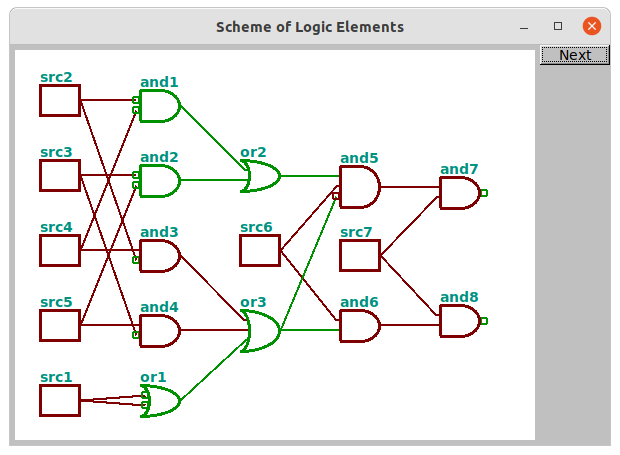
\includegraphics[width=0.6\textwidth]{images/logic_shapes.png}

  }
  \caption{Пример рисования логической схемы}
  \label{fig:logicshapes}
\end{figure}

Попробуем проанализировать задачу и продумать вопросы проектирования ещё раз, учитывая полученный опыт.



%%========================
\paragraph{Анализ задачи.}
%%========================
Нам дан пример схемы с~логическими элементами. Нужно ответить на~следующие вопросы и сформулировать задачу.
\begin{enumerate}
  \item Какова предметная область?
  \begin{itemize}
      \item Работаем с~элементами математической логики.
  \end{itemize}

  \item В~каком контексте нужно разработать программный код?
  \begin{itemize}
    \item Необходим программный код, который позволяет смоделировать работу данной схемы.
    \item Этот код вполне вероятно будет использован для~моделирования подобных схем.
    \item Было бы удобно, если бы моделирование схемы не~зависело от~способа отображения процесса её работы (рисования).
  \end{itemize}

  \item Анализ исходных данных:
  \begin{itemize}
    \item На~схеме изображены не~все существующие логические элементы.
    \item На~схеме нет циклов.
    \item Вместо логического отрицания используются отрицания на~выходах/входах логических элементов.
  \end{itemize}
\end{enumerate}



%%=========================
\paragraph{Проектирование.}
%%=========================
Необходимо предусмотреть гибкость разрабатываемого программного кода.
\begin{itemize}
  \item Расширение функционала не~должно вынуждать полностью переписывать исходный код.
  \item Разделение на~небольшие части, подзадачи, которые могут быть использованы независимо (принцип <<разделяй и властвуй>>).
  \item Необходимо предусмотреть наиболее удобные уровни абстракции.
\end{itemize}

\bigskip Выделим в~коде две части:
\begin{itemize}
  \item Код для~непосредственного моделирования работы схемы.
  \item Код для~отображения процесса работы схемы (рисование).
\end{itemize}

\bigskip Продумаем примеры того, как бы мы хотели видеть использование разработанного программного кода:
\begin{enumerate}
  \item Создание элементов.
  \begin{itemize}
    \item При~создании логического элемента нужно указать его тип (тип объекта), инвертирован ли его выход (по~умолчанию не~инвертирован), задать \code{callback}-функцию (по~умолчанию \code{nullptr}).
    \item При~создании источника логического значения (сигнала) нужно указать это значение (по~умолчанию \code{Signal::off}).
  \end{itemize}

  \item Соединение элементов.
  \begin{itemize}
    \item Соединений между логическими элементами гораздо больше, чем самих элементов.
    \item При~попытке сделать цикл в~схеме должно генерироваться исключение.
    \item Нужно предусмотреть (насколько это возможно) интуитивно понятный и лаконичный способ для~задания соединений.
    \item Удобно было бы соединять элементы по~цепочке.
    \item Будем использовать оператор~\code{>>} для~соединения элементов (\code{and1 >> or2}).
    \item Подключение на инвертированный вход вполне удобно смотрится с использованием оператора \code{\textasciitilde} (\code{or3 >> \textasciitilde{}and5}).
  \end{itemize}

  \item Изменение элементов.
  \begin{itemize}
    \item Для~задания логического значения источника удобно использовать оператор~\code{=} (\code{src1 = Signal::on}).
    \item Расчёт значений на~выходе каждого логического элемента должно происходить автоматически при~изменении состояния на~выходе элементов ниже по~цепочке.
    \item При~изменении состояния на~выходе элемента, этот элемент должен вызывать \code{callback}-функцию.
  \end{itemize}

  \item Получение значения на~выходе логического элемента.
  \begin{itemize}
    \item Оператор преобразования логического элемента в~значение \code{bool}.
  \end{itemize}

  \item Программный код для~отображения схемы и процесса её работы.
  \begin{enumerate}
    \item Нужно задавать только объекты, которые соответствуют логическим элементам на~схеме.
    \item Удобно создать класс-хранилище графических объектов \code{SchemeShape}.
    \item Отображение связей будет автоматическое, генерация объектов будет происходить в~\code{SchemeShape}.
    \item При~создании графических объектов нужно указать:
    \begin{itemize}
      \item на~какой схеме они расположены;
      \item какой логический элемент представляют;
      \item подпись (имя элемента);
      \item положение на~схеме.
    \end{itemize}
    \item Объект графического представления будет задавать \code{callback}-функцию для~элемента, который представляет.
    \item В~\code{callback}-функции будет происходить изменение цвета отображения элемента и связей.
  \end{enumerate}
\end{enumerate}



%%===================================
\section{Разработка логической части}
%%===================================
%%=========================================
\paragraph{Диаграмма наследования классов.}
%%=========================================
Набросаем иерархию классов, которые будут отражать наше представление о~логических элементах и взаимосвязях между ними.

\begin{center}\begin{tikzpicture}[node font=\ttfamily\small, >=Stealth]
    \graph [layered layout, components go right top aligned, edge=<-]
    {
        Scheme[text=blue];

        Element[align here, text=blue] ->[blue] {
            Source[text=blue],
            Operation[text=blue]
        };
        Operation ->[blue] {
            And[text=blue],
            Or[text=blue]
        };
    };

    \begin{scope}[on background layer]
        \node (Logic) [draw, blue, dashed, rounded corners,
        fit=(Element) (Source) (Scheme) (Operation) (And) (Or)] {};
        \node[text=blue, inner sep=0pt, above left=0pt of Logic.north west] {Logic};
    \end{scope}
\end{tikzpicture}\end{center}


%%=====================
\paragraph{Реализация.}
%%=====================
Объявление классов разместим в заголовочном файле \code{logic.h}, а реализацию методов и вспомогательных функций "--- в файле \code{logic.cpp}.

\bigskip
\todo{Ключевые моменты реализации будут размещены позднее.}


\clearpage
%%====================================
\section{Разработка графической части}
%%====================================
%%=========================================
\paragraph{Диаграмма наследования классов.}
%%=========================================
Для~графического изображения логических элементов нам придётся создать схожую иерархию классов. Отметим, что мы намерены отделить логику работы схем от~их рисования на~экране. Очевидно, мы могли бы отобразить нашу схему различными способами. Например, вывести структуру и состояние схемы в~консоль, нарисовать элементы с помощью графической библиотеки, и, наконец, сгенерировать файл с~описанием схемы для таких систем визуализации графов, как \name{GraphViz} или пакета \name{Tikz} системы вёрстки \LaTeX.

\begin{center}\begin{tikzpicture}[node font=\ttfamily\small, >=Stealth]
    \graph [layered layout, components go right top aligned, edge=<-]
    {
        Scheme[text=gray];

        Element[align here, text=gray, left=0pt] ->[gray] {
            Source[text=gray],
            Operation[text=gray]
        };
        Operation ->[gray] {
            And[text=gray],
            Or[text=gray]
        };

        Shape[as=Graph\_lib::Shape] -> ElementShape[text=blue] ->[blue] {
            SourceShape[text=blue],
            OperationShape[text=blue]
        };
        OperationShape ->[blue] {
            AndShape[text=blue],
            OrShape[text=blue]
        };
        Shape -> Rectangle[as=Graph\_lib::Rectangle] -> SchemeShape[text=blue];

        Element ->[edge=--, gray, dashed] ElementShape;

        { [same layer] Scheme, Element, ElementShape, SchemeShape };
    };

    \begin{scope}[on background layer]
        \node (Logic) [draw, gray, dashed, rounded corners, fit=(Element) (Source) (Scheme) (Operation) (And) (Or)] {};
        \node[text=gray, inner sep=0pt, above left=0pt of Logic.north west] {Logic};

        \node (GraphLib) [fit=(Shape) (Rectangle)] {};
        \node (ShapeLogic) [draw, blue, dashed, rounded corners, fit=(ElementShape) (SourceShape) (SchemeShape) (OperationShape) (AndShape) (OrShape)] {};
        \node[text=blue, inner sep=0pt, above right=0pt of ShapeLogic.north east] {Logic};
    \end{scope}
\end{tikzpicture}\end{center}



%%=====================
\paragraph{Реализация.}
%%=====================
Объявление графических классов и констант для управления стилем разместим в заголовочном файле \code{logic\_shapes.h}, а реализацию методов и вспомогательных функций "--- в файле \code{logic\_shapes.cpp}.

\bigskip
\todo{Ключевые моменты реализации будут размещены позднее.}



%%================
\WhatToReadSection
%%================
\textcite{Stroustrup:2016:ru}: \textbf{глава~15}



%%===============
\ExercisesSection
%%===============
\begin{exercise}
\item Выполните упражнения из \textbookref{главы~14} учебника.

\end{exercise}
